\documentclass[10pt]{article}
\usepackage[letterpaper,landscape,margin=0.65in]{geometry}
\usepackage{graphicx}
\usepackage{booktabs}
\usepackage{amsmath}
\usepackage[T1]{fontenc}
\usepackage{hyperref}
\hypersetup{pdftitle={FROB C5 finite-field factor-kernel audit},
  pdfsubject={EXP-FROB-91ee9c; three canonical field cells proved; archived code bridge open}}
\setlength{\parindent}{0pt}
\setlength{\parskip}{0.45em}
\title{FROB C5 finite-field factor-kernel audit}
\author{Validation audit, 22 October 2026}
\date{}
\begin{document}
\maketitle
\vspace{-2em}

\textbf{Scope.} Frozen \texttt{EXP-FROB-91ee9c} control C5;
Lean source commit \texttt{2143dda2b698cf6e3fb4bafbe853af7262e3ffba}.
These are mathematical statements about canonical degree-five finite fields.
They do not replay a scientific trial or establish an ECDLP performance claim.

\begin{center}
\begin{tabular}{llll}
\toprule
Base field & Nontrivial factors of $X^5-1$ & Lean kernel result & Sum dimension \\
\midrule
$\mathbf F_{11}$ & $X+2, X+6, X+7, X+8$ & four successive disjoint summands $=\ker\operatorname{Tr}$ & 4 \\
$\mathbf F_{13}$ & $X^4+X^3+X^2+X+1$ & sole factor kernel $=\ker\operatorname{Tr}$ & 4 \\
$\mathbf F_{19}$ & $X^2+5X+1, X^2+15X+1$ & disjoint sum $=\ker\operatorname{Tr}$ & 4 \\
\bottomrule
\end{tabular}
\end{center}

\textbf{Proof method.} Lean checks exact cyclotomic factorizations and
irreducibility. For $q=13,19$, it uses Mathlib's finite-field cyclotomic
factor criterion with $\operatorname{ord}_5(q)=4,2$; the $q=11$ factors have
degree one. Explicit coprimality certificates and Mathlib's polynomial-kernel
CRT give the direct sums. The prior finite-field theorem identifies
$1+F+F^2+F^3+F^4$ with the embedded trace and proves its kernel has dimension
four. Here $F$ is the $q$-power Frobenius on \texttt{GaloisField q 5}.

\textbf{Verification.} The three exact-source verifier receipts accompany the
report. They bind the target specifications, theorem source, pinned Lean
4.35.0-rc1 toolchain and dependency manifest. Each target axiom audit
passed; the full 8,971-job build passed and 612 theorem declarations used
standard axioms only. Independent semantic review remains pending.

\textbf{Archived matrix replay.} A separate plain-Python checker reads the
three frozen outputs, recomputes each $5\times5$ Frobenius matrix from the
recorded modulus, checks modulus/factor irreducibility and factor kernels,
directness and trace equality. The same gates reject a mutated matrix in all
three cells; the byte-exact receipt is included. A separate Lean certificate
now proves all 75 q-power matrix entries in the frozen quotient bases. A second
certificate proves direct factor-kernel sums and trace dimension four for the
exact recorded matrices. A third Lean certificate identifies the full
q-power quotient endomorphisms with those frozen matrices in their power bases.

\textbf{Negative control.} A separate Lean theorem proves
$X^5-1=(X-1)^5$ and non-squarefreeness over $\mathbf F_5$. This checks the
coprimality boundary; $q=5$ was not an archived core cell.

\textbf{Boundary.} Explicit quotient-kernel basis transport, historical Sage
code-path refinement, original source custody and independent review remain
open. The historical run
control, C8 and experiment success gate therefore remain open. No measured
value or performance dashboard curve changed.

\newpage
\begin{center}
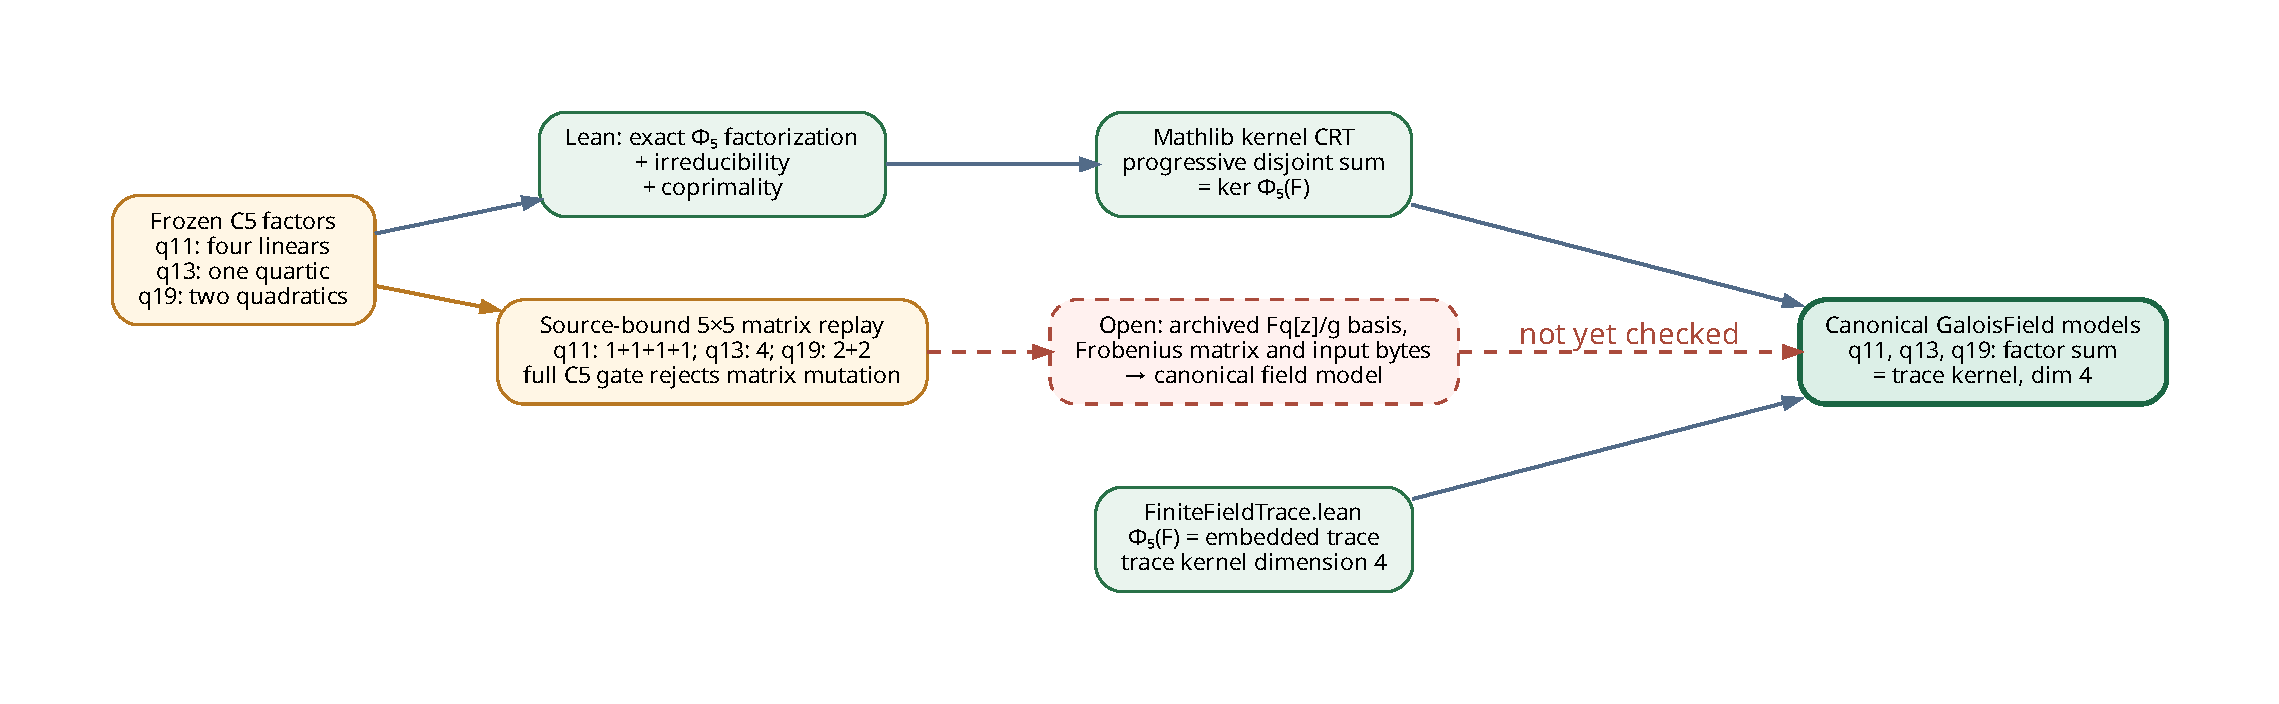
\includegraphics[width=\textwidth,height=0.82\textheight,keepaspectratio]{proof-figure.pdf}
\end{center}
\end{document}
